\documentclass[12pt]{article}

\usepackage{sbc-template}
\usepackage{graphicx,url}
\usepackage[utf8]{inputenc}
\usepackage[english]{babel}
\usepackage{booktabs}
\usepackage[hidelinks]{hyperref}

\sloppy

\title{Predicting Student Dropout in Brazil's Federal Network of the Northeast:\\
Calibration, Group Fairness and Retained Students}

\author{Maria Ingrid Xavier Sousa}

\address{Departamento de Computação -- Universidade Federal do Piauí (UFPI)\\
  Teresina -- PI -- Brazil
  \email{mariaingridxs03@gmail.com}
}

\begin{document}

\maketitle

\begin{abstract}
More than half of the enrollments that reach their expected end date in the federal institutes of
Northeast Brazil end in dropout. We trained a gradient boosting classifier on 178,484 enrollments
from the Nilo Peçanha Platform (2021--2023 editions), using only information available at enrollment, and
audited it for group fairness. The model reaches a test AUC of 0.829 (95\% CI 0.823--0.835), against 0.761 for
the historical dropout rate of the course, and is well calibrated across sex, race, income and age groups,
except for Indigenous students. Most of the gain from income and race comes from whether they were declared,
not from their values. A model trained only on one institute does not outperform the regional model, and a
sensitivity analysis shows that the usual exclusion of retained students leaves out 20\% of the cohort.
\end{abstract}

\begin{resumo}
Mais da metade das matrículas que chegam ao fim do prazo previsto nos institutos federais do Nordeste
termina em evasão. Treinamos um classificador de gradient boosting com 178.484 matrículas da Plataforma Nilo
Peçanha (edições 2021 a 2023), usando apenas informações disponíveis no ingresso, e avaliamos a justiça do
modelo entre grupos. O modelo atinge AUC de 0,829 no teste (IC 95\% 0,823--0,835), contra 0,761 da taxa
histórica de evasão do curso, e é bem calibrado entre grupos de sexo, cor/raça, renda e idade, exceto para
estudantes indígenas. A maior parte do ganho de renda e cor/raça vem de saber se foram declaradas, e não de
seus valores. Um modelo treinado só com um instituto não supera o regional, e uma análise de sensibilidade
mostra que excluir os alunos retidos, como é usual, deixa de fora 20\% das matrículas.
\end{resumo}

\section{Introduction}

Brazil's Federal Network of Professional, Scientific and Technological Education offers technical courses
(integrated with or after secondary school) and undergraduate programs. Dropout is one of its most persistent
problems: in the data used here, 58.4\% of the enrollments in the Northeast whose expected end date had passed
ended in dropout, around 51\% in technical courses and 79\% in undergraduate programs. 

A risk estimate available at enrollment could help pedagogical and student-assistance teams prioritize
follow-up early. But a model that misses the dropouts of one group, or flags another too often, can redirect support
unfairly~\cite{baker2022,kizilcec2022}.

This work asks two questions: using only enrollment data, can dropout be predicted better than with the historical
rate of the course, and are the model's errors and probabilities equally reliable across sex, race, declared income
and age? We use supervised classification on public microdata of the Nilo Peçanha Platform (PNP)~\cite{pnp}, with calibrated gradient boosting, a
group fairness audit and three further analyses: undeclared income and race, a regional versus a single-institution
model, and the exclusion of students still enrolled after the expected end (retained students).

\section{Related Work}

Several Brazilian studies predict dropout with PNP data.
\cite{oliveira2022} used the PNP enrollment microdata for 2019 and 2020, for the whole federal network and for the
Federal Institute of Paraíba (IFPB), with Random Forest for feature selection and classification. They report
accuracies between 0.86 and 0.90, but on yearly snapshots of the enrollment file, which mostly contain students
active in that year; we use the Academic Efficiency files, which follow complete cohorts to their final status, so
the figures are not directly comparable. On single campuses, \cite{barbosa2023} found XGBoost the best model for
the Federal Institute of Pernambuco, and \cite{cabral2025}, with PNP records of an IFPB campus from 2017 to 2023
and a prospective test on 2023, found Random Forest the best by AUC and recall. These studies focus on one institution or campus and on overall performance;
none of them examines whether the errors are evenly distributed across groups of students.

The fairness literature in education points exactly to that gap. \cite{baker2022} and \cite{kizilcec2022} review algorithmic bias in
education, and \cite{gardner2019} propose slicing analysis, evaluating the model separately for each group, as we
do. \cite{yu2021} found that adding protected attributes to a U.S. college dropout model did not
change overall performance and only marginally improved fairness. 
Finally, when base rates differ, a calibrated model cannot also equalize error rates such as the false positive
rate~\cite{kleinberg2017,chouldechova2017,hardt2016}.

\section{Methodology}

\subsection{Data}

We used the Academic Efficiency microdata of the PNP~\cite{pnp}, editions 2021, 2022 and 2023, published under the
Open Data Commons Open Database License. Each edition contains one row per enrollment in a course cycle whose
expected end date fell in the previous year, with the final status of the student: completed, dropped out or still
enrolled (retained). We kept the Northeast and technical, technology, teacher-education and bachelor's courses;
internal transfers were not counted as dropout. The label is 1 for dropout and 0 for completion; retained students were excluded from
the main base because their outcome is still unknown, and analyzed separately (Section~\ref{sec:retained}). The base has 178,484 enrollments from 23 institutions, 219 campuses and 203 courses, with
58.4\% dropout (57.9\%, 60.9\% and 56.4\% by edition).

The age at enrollment was recomputed from the age on December 31 of the edition year. Institution names
changed between editions (acronyms in 2021--2022, full names in 2023), so the name also encoded the edition; after
standardizing them, the test AUC fell from 0.832 to 0.829, the honest value, since the edition is unknown at
prediction time.

\subsection{Features and protocol}

The model uses 19 features known at enrollment: institution, campus, state, course name, course type, offer type
(integrated, concurrent, subsequent, adult education), modality, shift, technological area and sub-area, funding
program, workload, expected duration, month of entry, age at entry, sex, race, and two indicators of whether income
and race were left undeclared. The enrollments were randomly split into training (70\%, 124,938), validation (20\%,
35,697) and test (10\%, 17,849) sets, stratified by edition and label with a fixed seed (42). Models were fitted on
training data, tuned, calibrated and thresholded on validation; the test set was used once, at the end.

\subsection{Models}

The references are the majority class; the historical dropout rate of the course in the campus, smoothed toward the
rate of the course type (a rule an institution could compute without machine learning); logistic regression with
one-hot encoding; and gradient boosting variants without the missingness indicators or with the declared income and
race values. The main model is scikit-learn's histogram gradient boosting~\cite{pedregosa2011}, with native categorical features, early stopping and L2 regularization of 1.0.
Twelve combinations of learning rate (0.05, 0.1), maximum leaves (15, 31, 63) and minimum samples per leaf (20, 100)
were compared by validation AUC; the final model uses 0.05, 63 and 100, with 519 trees. Probabilities were
calibrated with isotonic regression~\cite{zadrozny2002} on the validation set. Because the levels have very different
base rates, the alert threshold was chosen per level (technical 0.52, undergraduate 0.80) by maximizing balanced
accuracy on the validation set.

\subsection{Evaluation}

We report AUC with 95\% bootstrap confidence intervals, the Brier score, and accuracy and balanced accuracy at the
chosen thresholds. For fairness, each group of sex, race, declared income, age at entry and course level is evaluated
separately (slicing analysis~\cite{gardner2019}): calibration error (mean predicted minus observed dropout),
recall and false positive rate~\cite{hardt2016}. Two attribute decisions were taken with criteria fixed before
running the comparison: race was adopted as an input if it reduced the calibration error of Indigenous students by
more than 2 points while losing less than 0.002 of AUC, and the declared income bracket under the same rule applied
to income groups.

\section{Results and Discussion}
\label{sec:results}

\subsection{Overall performance}

Figure~\ref{fig:models} compares the models on the test set. The final model reaches an AUC of 0.829
(0.823--0.835) and a Brier score of 0.165, against 0.761 and 0.195 for the historical course rate and 0.788 and
0.183 for logistic regression. With the per-level thresholds it classifies 72.5\% of the test enrollments correctly
(balanced accuracy 72.4\%), against 68.0\% for the historical course rate. Accuracy is not uniform: in the 10\% of
students on whom the model is most confident it is right 88\% of the time, and 85\% in the top 30\%. The learning curve was still rising (validation AUC 0.819 with half of the
training data, 0.831 with all of it), so more data is likely to help.

\begin{figure}[ht]
\centering
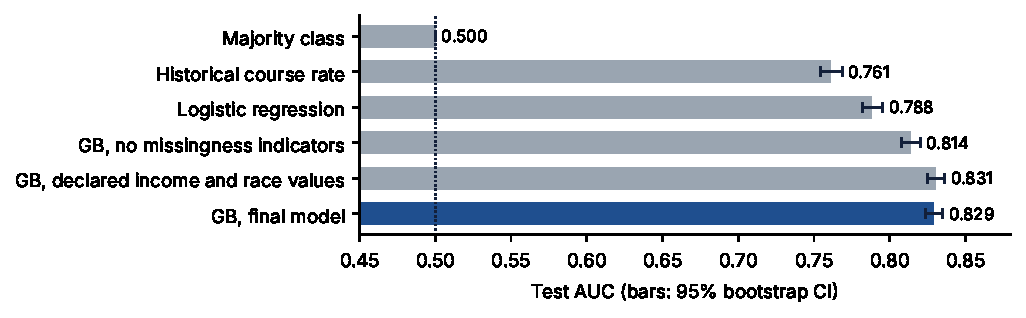
\includegraphics[width=.6\textwidth]{fig_models.pdf}
\caption{Test AUC of the references and of the gradient boosting (GB) variants, with 95\% bootstrap intervals.}
\label{fig:models}
\end{figure}

\subsection{Undeclared income and race}

Missing information was the strongest socio-economic signal. In the 2023 enrollment file (entrants from 2015 to 2023),
the share without declared income among students still enrolled is similar for every entry year (24\% for 2023
entrants), so income is recorded, or not, at enrollment and does not leak the outcome. Within the same institution, students without declared
income dropped out more in 15 of 16 comparable institutions (median difference of 11.9 points), and students without
declared race in 15 of 16 (13.8 points). On validation, the two missingness indicators alone added 0.018 of AUC,
106\% of the gain of the full declared values, which add nothing ($-0.004$) among students who declared both. Race was adopted as an input because it reduced the underestimation of the risk
of Indigenous students from 5.8 to 3.0 points on validation (10.4 to 6.6 on test) at a cost of 0.0005 of AUC. The
declared income bracket was not adopted: the model was already calibrated across income brackets (largest error 3.3
points), and the bracket reduced it by only 1.2 points.

\subsection{Group fairness}

Figure~\ref{fig:fairness} shows the slicing analysis of the final model. Calibration is good for almost every group
(errors within $\pm$3 points). Error rates, however, differ: men have higher recall (77.1\% vs.\ 67.5\%) but also more false
positives (33.6\% vs.\ 23.1\%), and the same pattern separates students with and without declared income. These
differences follow from different base rates, as predicted by \cite{kleinberg2017} and \cite{chouldechova2017}: a
calibrated model gives more alerts where dropout is more frequent. Two groups need attention: Indigenous students
are still underestimated by 6.6 points (98 test enrollments), and only 39\% of the dropouts of students aged 17 or
less are flagged, so the model should not be their only screening tool.

\begin{figure}[ht]
\centering
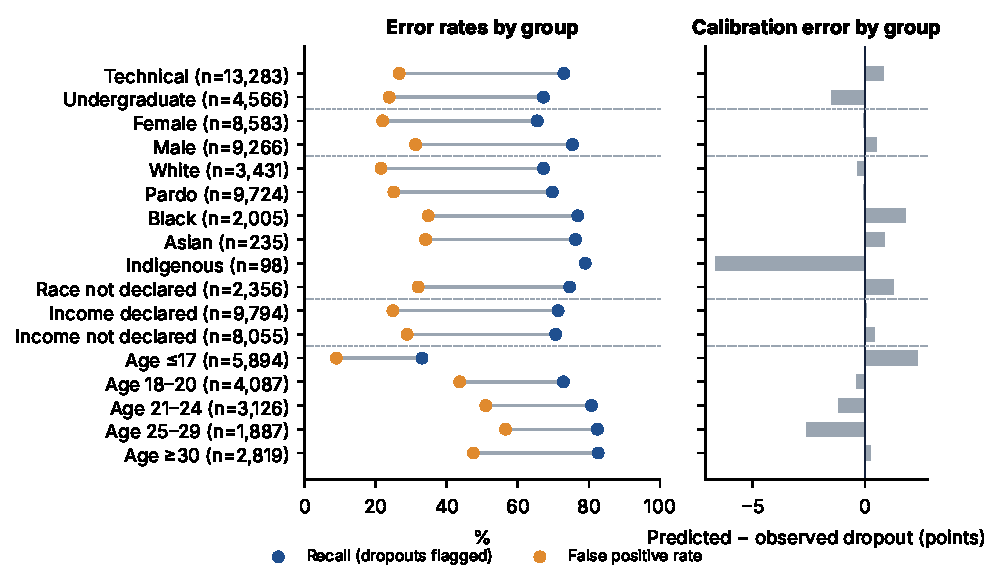
\includegraphics[width=.74\textwidth]{fig_fairness.pdf}
\caption{Slicing analysis of the final model on the test set, with per-level thresholds. The false positive rate
of Indigenous students is omitted because the group has fewer than 30 students who completed.}
\label{fig:fairness}
\end{figure}

\subsection{Regional model or institution-specific model?}

For the Federal Institute of Piauí (IFPI), with 13,066 training and 1,952 test enrollments, we compared the
regional model with a model trained only on IFPI data, the regional model recalibrated on IFPI, and the regional model
without institution and campus (Table~\ref{tab:ifpi}). All four tie (paired differences include zero), and the
regional model is already calibrated for IFPI (mean error of 0.8 points). Since removing institution and campus does
not hurt, differences between institutions seem to come from their mix of courses and students; a single regional
model is adequate.

\begin{table}[ht]
\centering
\caption{Models evaluated on the IFPI test enrollments (n = 1,952). Difference: paired bootstrap, 95\% CI.}
\label{tab:ifpi}
\small
\begin{tabular}{lcc}
\toprule
Model & AUC & Difference from regional \\
\midrule
Regional (Northeast) & 0.807 & -- \\
IFPI only & 0.806 & $-0.001$ ($-0.007$ to $+0.005$) \\
Regional, recalibrated on IFPI & 0.808 & $+0.001$ ($-0.001$ to $+0.002$) \\
Regional without institution and campus & 0.810 & $+0.002$ ($-0.006$ to $+0.010$) \\
\bottomrule
\end{tabular}
\end{table}

\subsection{Retained students}
\label{sec:retained}

Retained students are usually excluded from dropout studies~\cite{oliveira2022}, as in our main model. They are
44,723 enrollments, 20.0\% of all whose expected end had passed (29.2\% in undergraduate programs), and resemble
dropouts: median age at entry of 21, as for dropouts (17 for graduates), and an average predicted risk of 65\%, close
to dropouts (72\%) and far from graduates (40\%). We trained a
second model for ``did not complete on time'' (dropout or retained). Both perform alike on their own question
(Table~\ref{tab:retained}), but the second has smaller gaps between groups: the recall gap between
students with and without declared income falls from 17.3 to 11.9 points, the false positive gap between levels from
6.4 to 1.4, and the calibration error for Indigenous students from $-6.6$ to $-4.1$. Excluding retained students
therefore probably underestimates non-completion and slightly increases group disparities. We kept dropout as the
main target because it is a definitive outcome.

\begin{table}[ht]
\centering
\caption{Each model evaluated on its own question in the test set.}
\label{tab:retained}
\small
\begin{tabular}{lcc}
\toprule
 & Dropout (main) & Did not complete on time \\
\midrule
Positive rate & 58.4\% & 66.7\% \\
AUC & 0.829 & 0.826 \\
Balanced accuracy & 72.4\% & 72.1\% \\
Recall / false positive rate & 72.8\% / 28.0\% & 70.7\% / 26.4\% \\
\bottomrule
\end{tabular}
\end{table}

\textbf{Limitations and risks.} The estimate describes students with a similar profile, not the future of a person;
it uses no grades or attendance, the cohorts went through the COVID-19 pandemic, and it covers only the Northeast. It
must be used to offer support, never to deny seats, scholarships or rights.

\section{Conclusion}

With enrollment data only, a calibrated gradient boosting model predicts dropout clearly better than the historical
course rate (AUC 0.829 vs.\ 0.761), and a regional model serves an institute as well as a local one. Probabilities
are reliable across groups, but error rates follow base rates, Indigenous students remain underestimated and young
technical students are hard to flag. The strongest socio-economic signal is whether income and race were declared,
and excluding retained students hides a fifth of the cohort. Future work
includes first-semester grades and attendance, more editions and regions, temporal validation and fairness-aware
thresholds. A demonstration website computes the estimate in the browser and explains it with group Shapley
values~\cite{lundberg2017}.

\section*{Data and Code Availability}

\noindent Dataset (raw PNP microdata and cleaned base, ODbL):\\
\url{https://www.kaggle.com/datasets/mariaingridxavier/evasao-na-rede-federal-do-nordeste-pnp-2021-2023}\\
Notebook, executed end to end:\\
\url{https://www.kaggle.com/code/mariaingridxavier/evasao-na-rede-federal-do-ne-previsao-e-vies}\\
Code: \url{https://github.com/mingridxs/evasao-rede-federal-ne}\\
Demonstration website: \url{https://mingridxs.github.io/evasao-rede-federal-ne/}

\section*{Use of Large Language Models}

Claude (Anthropic) was used to search for datasets and documentation, suggest the experimental design, generate
and debug code, build the demonstration website, and draft and translate the text of this paper. All runs were
performed by the author on the real data; the author checked every number in the paper against the notebook outputs
and revised the text. Representative prompts include ``can you write code to process the data and keep only what
matters?'' (with a screenshot of the PNP spreadsheet) and ``can't we improve the model's result?''.

\bibliographystyle{sbc}
\bibliography{referencias}

\end{document}
